\chapter{Auswertung, Fehlerrechnung und Diskussion der Messergebnisse}
\section{Aufgabe 1: Einfluss der Spitzengeometrie}
\begin{figure}[H]
    \centering
    \includegraphics[width=110mm,scale=0.5]{Rasterkraftmikroskop/include/fälle.png}
    \caption{Zu behandelnde Fälle} 
    \label{fig:faelle}
\end{figure}
Der Einfluss der Spitzengeometrie wurde bereits in Kapitel \ref{chap:aufloesung} behandelt. Im Rahmen dieser Aufgabe sollen die Scanlinien zu den in Abbildung \ref{fig:faelle} angegebenen Fällen aufgezeigt werden. Diese sind in Abbildung \ref{fig:scanlinien} sichtbar. 


Es ist ersichtlich, das die Geometrie der Spitze großen Einfluss auf die Scanlinien hat. Merkmale der Probenoberfläche können nur korrekt abgebildet werden, wenn Ausmaße größer als die der Spitze sind. So kann zum Beispiel Fall c nicht richtig abgebildet werden. Spitzenartefakte in der Scanlinie lassen sich durch Änderung der Scanrichtung einfacher identifizieren, jedoch ist eine genaue Zuordnung meistens nicht möglich.   
\begin{figure}[H]
    \centering
    \includegraphics[width=110mm,scale=0.5]{Rasterkraftmikroskop/include/scanlinien.png}
    \caption{Die entstehenden Scanlinien} 
    \label{fig:scanlinien}
\end{figure}
\section{Aufgabe 2: Einfluss des Spitzenradius}
Unter der Vorraussetzung, das sowohl Spitze als auch Topographiedetail Halbkugeln mit Radius $R$ bzw. $r$ sind, lässt sich über den Satz des Pythagoras die folgende Gleichung aufstellen
$$R^2 + R_{mess}^2 = (R+r)^2$$
wobei $R_{mess}$ der gemessene Radius des Topographiedetail ist. 
Woraus folgt
$$R = \frac{R_{mess}^2 - r^2}{2r}$$
Will man nun eine Vergrößerung des Messergebnisses von höchstens \SI{10}{\%}, setzt man für $R_{mess} = 1,1 r$ ein. 
Damit ergibt sich ein Detailradius von $$R = 0,105r, r = 9,524R$$
Das Detail muss somit einen Radius von mindestens $9,524\cdot R$ haben, damit das Messergebnis um weniger als \SI{10}{\%} vergrößert wird.


\section{Aufgabe 3: Federkonstante des Cantilevers}
Die Federkonstante des Cantilevers kann mithilfe der Gleichung $$c_n = \frac{E\cdot w\cdot t^2}{4 \cdot l^3}$$ bestimmen. Dabei ist $E$ das Elastizitätsmodul, $w$, $t$ und $l$ die Dimensionen des Cantilevers. 
Mit den gegebenen Daten $E = \SI{1,69 }{\cdot 10^{11}\frac{N}{m^2}}, l = \SI{350 \pm 5}{\mu m}, w = \SI{35 \pm 3}{\mu m}, t = \SI{1 \pm 0.3}{\mu m}$ und gaußscher Fehlerfortpflanzung ergibt sich die Federkonstante zu
$$c_n = \SI{0,03 \pm 0,02}{\frac{N}{m}}$$
was mit dem im Datenblatt gegebenen Wert übereinstimmt. 

\section{Aufgabe 4: Vermessen des Lochgitters}
\label{chapter:Aufgabe4}
In Abbildung \ref{fig:lochgitter} ist das Topographie-Signal und das Top-Bottom-Signal sichtbar. Die Struktur des Lochgitters ist gut erkennbar, allerdings erscheinen die Rechtecke leicht verzerrt. Dies tritt wahrscheinlich aufgrund der Geometrie der Spitze auf, welche die Auflösungsgrenze beschränkt. Die unterschiedliche Einfärbung der Stege im Topographie-Signal ergibt sich dadurch, das die Höhe immer im Verhältnis zum Mittel aller Höhenwerte eines Scans berechnet wird. Da in x-Richtung gescannt wurde, ergibt sich entlang der waagerechten Stege ein praktisch konstanter Höhenwert, der auch dem Mittelwert entspricht. Wird über Zeilen gescannt in denen sich Löcher und Stege abwechseln, ist das Mittel dieser Höhenwerte nicht mehr gleich dem waagerechten Stege, wodurch die senkrechten Stege sehr viel hellen eingefärbt sind. Entlang der Stege lassen sich einige Artefakte erkennen, was darauf schließen lässt das die Oberfläche des Lochgitters nicht glatt ist und eventuell durch diese und vorherige Messungen beschädigt wurde. In beiden Signalen ist links ein Artefakt zu sehen, welches darauf schließen lässt das der Cantilever zu Beginn des Scans nach dem Aufsetzen auf der Probe eine stotternde Bewegung ausgeführt hat, bis die Haftreibung völlig überwunden wurde.\\
\begin{figure}[t]
    \centering
    \includegraphics[width=110mm,scale=0.5]{Rasterkraftmikroskop/Daten/A4.png}
    \caption{Topograhie-Signal (links) und Top-Bottom-Signal (rechts) des Lochgitters} 
    \label{fig:lochgitter}
\end{figure}
\begin{table}[t]
    \centering
    \caption{Ermittelte Dimensionen des Lochgitters}
    \begin{tabular}{cc}
    \hline
        Breite $b$ in $\mu$m& $5,36 \pm 0,12$\\
        Länge $l$ in $\mu$m& $5,05 \pm 0,21$\\
        Höhe $h$ in nm& $226 \pm 2,24$\\\hline
    \end{tabular}
    
    \label{tab:lochdim}
\end{table}
\begin{table}[H]
    \centering
    \caption{Korrekturfaktoren der Achsen}
    \begin{tabular}{cc}
    \hline
        $k_b$ & \SI{-6,9}{\%} \\
        $k_l$ &  \SI{-1}{\%}\\
         $k_h$ & \SI{-10,02}{\%}\\\hline
    \end{tabular}
    
    \label{tab:korrs}
\end{table}
Mithilfe der bereitgestellten Software konnten die Ausmaße der Löcher bestimmt werden, deren Mittelwert und Standartabweichung in Tabelle \ref{tab:lochdim} gegeben sind. Nach Herstellerangaben haben die Löcher die Ausmaße $\SI{5}{\mu m} \cdot \SI{5}{\mu m} \cdot \SI{200}{nm}$. Die ermittelten Werte liegen somit in der gleichen Größenordnung wie die Herstellerangaben, beinhalten diese allerdings nicht in ihren Unsicherheitsbereichen. Anhand dieser Diskrepanz lassen sich nun Korrekturfaktoren für jede Achse berechnen. Diese sind in Tabelle \ref{tab:korrs} gegeben.
\\Die Kalibrierung mit nur einem Korrekturfaktor pro Auslenkungsrichtung hat den Nachteil, das nicht lineare Effekte nicht ausreichend berücksichtigt werden können. Einer dieser ist zum Beispiel die Scannerauslenkung, welche nicht immer linear mit der Spannung verläuft. \\Eine regelmäßige Nachkalibrierung des Scannerröhrchens ist notwendig, weil sich das aufgeprägte elektrische Dipolmoment des Scanners mit der Zeit verschlechtert, indem sich die Ausrichtung der Dipole ändert. Damit ändert sich auch die mechanische Geometrieänderung pro angelegter Spannung. 

\section{Aufgabe 5: Kraftabstandkurve am Lochgitter}
Im Spektroskopiemodus wird eine Kraftabstandkurve am Lochgitter aufgenommen, einmal bei Annäherung der Spitze zur Probe und einmal bei Entfernung. Die beiden Kurven sind in Abbildung \ref{fig:kraftabstand} zu sehen.
\begin{figure}[]
    \centering
    \includegraphics[width=110mm,scale=0.5]{Rasterkraftmikroskop/include/A5_komb.png}
    \caption{Kraftabstandkurve bei Annäherung (links) und Entfernung (rechts) der Spitze} 
    \label{fig:kraftabstand}
\end{figure}
Der erwartete snap-in ist im rechten Teil der Abbildung nicht zu sehen, und somit wohl sehr gering. Der erwartete snap-off scheint außerhalb des gemessenen Bereichs stattzufinden und ist somit nicht auf Abbildung \ref{fig:kraftabstand} sichtbar. 
Die Sensitivität ist durch die inverse Steigung der Kraftabstandskurve im Bereich  in diesem Fall muss sie durch Äbschätzung der Steigung anhand von zwei Punkten bestimmt werden. Die gewählten Punkte sind in Tabelle \ref{tab:koords} angegeben. 
\begin{table}[]
    \centering
    \caption{Ausgewählte Punkte bei Entfernung der Spitze}
    \begin{tabular}{c|c}
        Spannung &  z-pos\\\hline
        \SI{1.40 \pm 0.20}{V}& \SI{100}{nm}\\ 
        \SI{-4.10 \pm 0.20}{V} & \SI{-99,8}{nm} \\\hline
    \end{tabular}
    
    \label{tab:koords}
\end{table}
Daraus ergibt sich eine Steigung von $m = \SI{0.0275\pm 0,0014}{\frac{V}{nm}}$ und eine Sensitivität von $ S =\SI{36.3\pm 1.9}{\frac{nm}{V}}$
Die Auflagekraft lässt sich dann über $$F_n = c_n \cdot S\cdot \Delta U$$
berechnen, wobei $\Delta U$ die Setpointspannung von 109,01V ist. 
Damit ergibt sich $$F_n = \SI{1,2\pm0,8}{10^{-7} N}$$ was im erwarteten Bereich von $\SIrange{e-7}{e-10}{N}$ liegt.
Die Adhäsionskraft wird bestimmt durch 
$$F_{adh} = c_n \cdot \Delta z$$
berechnet, wobei $\Delta z$ der Abstand zwischen snap-off und snap-on ist. Da der snap-off nicht gemessen wurde, kann die Adhäsionskraft hier nicht bestimmt werden.\\Während der Berechnung wurden die Unsicherheiten auf $c_n$ und $S$ mit gaußscher Fehlerfortpflanzung beachtet.

\section{Aufgabe 6: Aussehen von Kraftabstandkurven}

Das Aussehen von Kraftabstandskurven in Medien kann von verschiedenen Effekten beeinflusst werden. \\

In Luft muss erscheint eine Hysterese zwischen snap-in und snap-off aufgrund der auftretenden Kapillarkräfte, da die Probe in Luft typischerweise von einem Adsorbatfilm aus Wasser bedeckt wird. In UHV oder Flüssigkeit ist diese Hysterese kleiner, da der Adsorbatfilm auf der Probe in UHV dünner ist oder in Flüssigkeiten nicht existiert. Bei Messungen in Luft muss darauf geachtet werden, das der Adsorbatfilm tatsächlich von der Spitze durchdrungen wird um die Topographie der Probe zu messen. 

In Flüssigkeiten müssen hydrodynamische Effekte beachtet werden, welche die Kraftabstandskurven beeinflussen. 

Um die Spitze vor abruptem Aufprall auf die Probenoberfläche zu schützen, ist eine Messung in UHV oder Flüssigkeit sinnvoll. 

Eine weiche Probe liefert typischerweise eine flachere und breitere Kraftabstandskurve als eine harte Probe. Aus den gemessenen Kraftabstandskurven kann die Elastizität der Probe ermittelt werden. 

Eine größere Cantileverfederkonstante würde zu schärferen Features in den Kraftabstandkurve führen, eine weichere Feder würde diese verbreitern.


\section{Aufgabe 7: Untersuchung einer CD-Oberfläche}

In Abbildung \ref{fig:CD} ist die Messung der Schreibfolie einer CD zu sehen. Die Probe wurde selbst angefertigt, indem die Schreibfolie einer CD mittels Klebeband abgezogen wurde. 
\begin{figure}[]
    \centering
    \includegraphics[width=110mm,scale=0.5]{Rasterkraftmikroskop/Daten/A7.png}
    \caption{Topographie-Signal (links) und Top-Bottom-Signal (rechts) der Schreibfolie einer CD} 
    \label{fig:CD}
\end{figure}
Auf der Abbildungen sind Verzerrungen und Artefakte deutlich sichtbar. Es ist möglich sich in dem Klebestreifen, auf dem die Probe befestigt war ein Knick befand, sodass die Probe sich während des Messung unter Einfluss des Cantilevers bewegen konnte. 
Die Breite und Tiefe/Höhe der Pits und Lands, sowie der Abstand der Tracks wurde durch die bereitgestellte Software ermittelt. Dabei wurde nur der untere Bereich des Top-Bottom-Signals verwendet, der frei von Artefakten oder Verzerrungen ist. 
Dafür wurden mehrere Messpunkte aufgenommen, die Mittelwerte und Standartabweichung von diesen Messungen sind in Tabelle \ref{tab:CDTAB} gegeben. 

\begin{table}[]
    \centering
    \caption{Ermittelte Topographie}
    \begin{tabular}{ccc}
        Messgröße & Mittelwerte & Standartabweichung \\\hline
        Breite & $\SI{1,08}{\mu m}$& $\SI{0,16}{\mu m}$\\
        Tiefe & \SI{161.6}{nm}&\SI{23.5}{nm} \\
        Spurenabstand & $\SI{0,65}{\mu m}$& $\SI{0,06}{\mu m}$\\\hline
    \end{tabular}
    
    \label{tab:CDTAB}
\end{table}

Die optimale Topographie der Schreibfolie einer CD lässt sich aus der Wellenlänge der infraroten Laserdiode berechnen, welche benutzt wird um Daten auszulesen. Typischerweise strahlen die verwendeten Laserdioden Licht bei einer Wellenlänge von $\lambda = \SI{780 \pm 10}{nm}$ ab. CDs bestehen aus Polycarbonat mit einem Brechungsindex von $n = 1,59$. Somit verkürzt sich die Wellenlänge des Abtastlasers zu 
$$\lambda_{CD}  = \frac{\lambda}{n} = \SI{491 \pm 6}{nm}$$. Beim Auslesen der Daten macht man sich die destruktive Interferenz zwischen dem Licht von Pits und Lands zu Nutze, welches als Schwankung der Lichtintensität an einer Fotodiode registriert wird. Um destruktive Interferenz zu erreichen, muss der Gangunterschied zwischen den beiden Teilstrahlen eine halbe Wellenlänge betragen. Da an die Teilstrahlen an der Oberfläche der Schreibfolie reflektiert werden, bevor sie zur Fotodiode gelangen, muss der Höhenunterschied der Lands und Pits ein Viertel der Wellenlänge betragen, damit destruktive Interferenz zustande kommt. 
$$\Delta h_{opt} = \frac{\lambda_{CD}}{4} = \SI{122,6 \pm 1,6}{nm}$$
Wendet man den in Aufgabe \ref{chapter:Aufgabe4} ermittelten Korrekturfaktor auf den durch Messung ermittelten Wert an, erhält man
$$\Delta h_{korr} = \SI{145 \pm 21}{nm}$$
Die Unsicherheitsbereiche der ermittelten Höhe und der berechneten optimalen Höhe überschneiden sich nur wenig, allerdings liegen die Mittelwerte in der gleichen Größenordnung. Es ist möglich das diese Abweichung durch die Verzerrungen der Messungen zustande kommen, oder durch eine unzureichende Bestimmung des Korrekturfaktors.
Auf den Spurenabstand und die Breite der lassen sich die Korrekturfaktoren nicht anwenden, da diese jeweils für die x-\&y-Achse gelten, die Tracks, Pits und Lands allerdings in der x-y-Ebene verdreht sind. 

\section{Aufgabe 8: Gedankenexperiment}

Im folgenden soll für das beschriebene Gedankenexperiment das Torsionssignal gegen die Scankoordinate aufgetragen werden. Dabei soll darauf geachtet werden, das die Spitzenkoordinate nicht mit der Scankoordinate übereinstimmt. 
Wichtig sind hier besonders folgende Bereiche:
Zu beginn des Scans überwiegt die Haftreibung, was zu einem hohen Ausschlag des absoluten Torsionssignals führt, welches schnell wieder abfällt, da die Haftreibung in die geringe Gleitreibung übergeht. 
Beim Übergang von Oberflächen verschiedener Reibung gibt es einen schnellen Abfall bzw Anstieg des absoluten Torsionsignals auf das Niveau des Torsionssignals bei Gleitreibung der neuen Oberfläche. Bei Übergang von geringer Reibung zu hoher Reibung kommt es zudem noch zu Haftreibung, welche das absolute Torsionssignal zum Ausschlagen bringt. Bei Richtungsumkehrung wird der Cantilever nicht neu aufgesetzt, sodass das Torsionssignal langsam das Vorzeichen ändert. 
Abbildung \ref{fig:gedankenex} wurde unter Berücksichtigung dieser Merkmale erstellt. 

\begin{figure}[H]
    \centering
    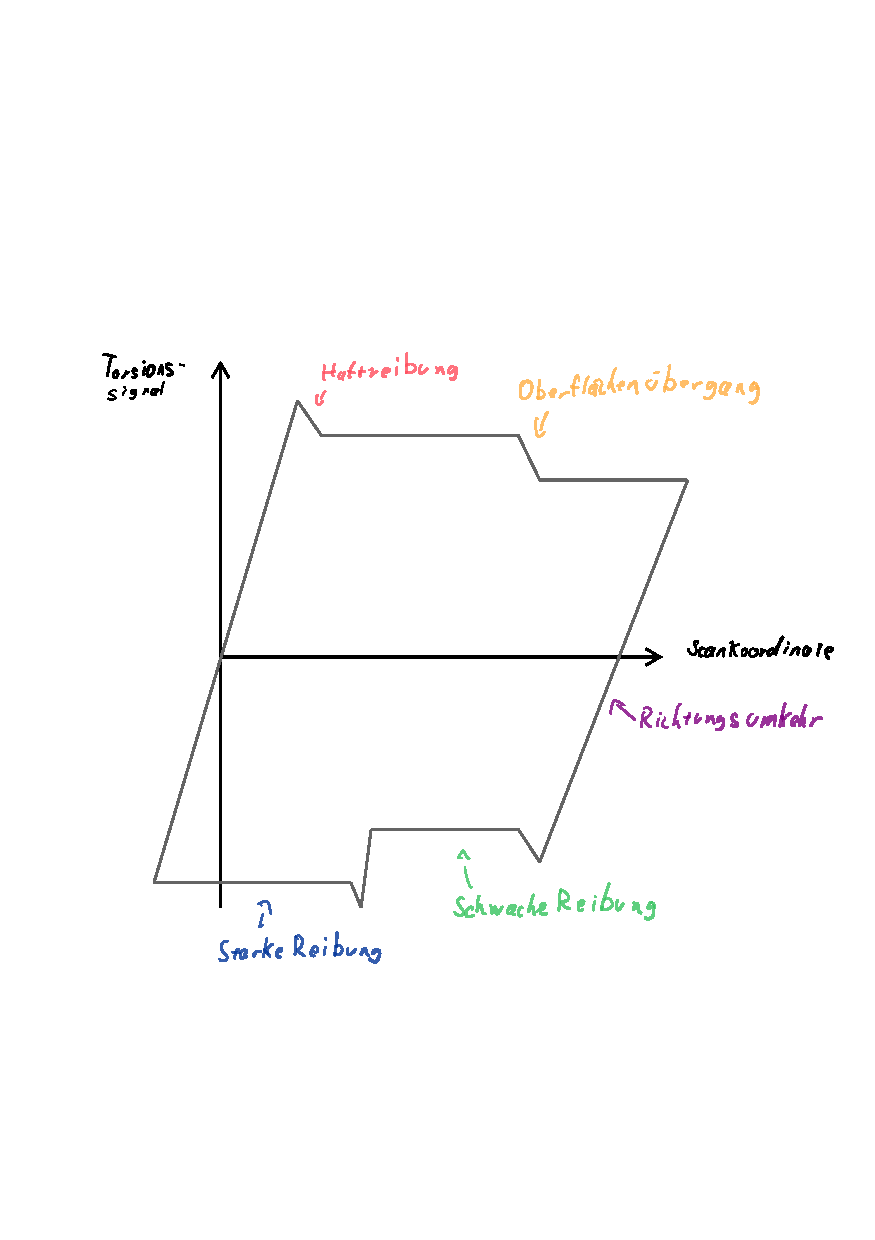
\includegraphics[width=110mm,scale=0.5]{Rasterkraftmikroskop/include/bild-3.png}
    \caption{Torsionssignal über Scankoordinate skizziert} 
    \label{fig:gedankenex}
\end{figure}

\section{Aufgabe 9: Messung einer Polymerblend-Probe}

Die Messung der Probe ist in Abbildung \ref{fig:poly} sichtbar. 
Die Probe besteht offensichtlich aus zwei Polymeren mit verschiedenen Reibungskoeffizienten. 

\begin{figure}[b]
    \centering
    \includegraphics[width=110mm,scale=0.5]{Rasterkraftmikroskop/Daten/A9.png}
    \caption{Reibungssignal der Polymerblend-Probe im Vorwärts- (links) und Rückwärtsscan (rechts)} 
    \label{fig:poly}
\end{figure}

Die Messungen des Vorwärts- und Rückwärtsscans sind in der Intensität gespiegelt, da der Cantilever jeweils in die andere Richtung gedreht ist. In beiden Abbildungen sind zu Beginn der Messung, also in Vorwärtsrichtung links im Bild, bei Rückwärtsrichtung rechts im Bild Artefakte zu sehen. Dieses stottern der Spitze entsteht durch die Haftreibung, welche der Richtungsumkehr folgt. Dieses Verhalten ist auch in der Messung der CD aufgetreten. \\
Eine Übersprechung des Reibungssignals in das Topographiesignal entsteht, wenn eine Verdrehung des Cantilevers nicht klar von einer Verbiegung zu unterscheiden ist. Das richtige Topographiesignal kann man dennoch ermitteln, indem man die Topographie in Vorwärts- und Rückwärtsrichtung misst und deren Differenz bildet. Die lateralen Kräfte wechseln bei Richtungsänderung das Vorzeichen, sodass sich diese durch die Differenzbildung genau aufheben. 

Unter Piezocreep versteht man das die Verzerrung des Piezoröhrchens, wodurch bei Start der Messung die tatsächliche Krümmung des Piezoröhrchens der erwarteten nicht nachkommt, was sich durch eine Verzerrung der Messung am Startrand sichtbar macht. In unserem Fall ist der Piezocreep nicht deutlich sichtbar. 

Zwischen Topographie- und Reibungsbildern kann durch Betrachtung der Vorwärts- und Rückwärtsscans unterschieden werden. Die Signale der Reibungsbilder sind in den Scanrichtungen zueinander invertiert.